\documentclass[11pt]{article}
\usepackage{cite}
\usepackage{amsthm}
\usepackage{amsfonts}
\usepackage{graphicx}
\usepackage{tikz}
\usetikzlibrary{calc}

\begin{document}

\newtheorem{mydef}{Definition}
\title{Symbolic Model checking of Timed Automata using LTSmin}
\author{Sybe van Hijum}
\date{\today}
\maketitle

\tableofcontents

\section{Introduction}
Timed Automata~\cite{Alur1994183} are a widely used modelling formalism. A recent usage of this formalism is the modelling of biological signalling pathways~\cite{DBLP:conf/bibe/SchivoSWCVKLPP12}. This leads however to large state spaces, and sometimes to models that are too large to handle by conventional methods. Therefore better model checking techniques for timed automata, that can handle larger state spaces are needed. We look into symbolic algorithms for timed automata.

BDDs(Binary Decision Diagrams)~\cite{?} and variations like LDDs(List Decision Diagrams)~\cite{so62465} and MDDs(Multi-valued Decision Diagrams)~\cite{129849} have proven their value in model checking algorithms. Due to advances in this field, models with much larger state spaces can be explored on the same machine. This progress has not been translated directly to more efficient methods for Timed Automata. Several methods have been proposed, like CDDs(Clock Difference Diagrams)~\cite{BRICS19491}, CMDs(Constraint Matrix Diagrams)~\cite{5702245}, CRDs(Clock Restriction Diagrams)~\cite{crds} and DDDs(Difference Decision Diagrams)~\cite{ddds, ddd-datastructure-99}. All of these methods show some extra difficulties or limitations over BDDs. Also after their introduction they have not been developed further.

LTSmin~\cite{eemcs18152,ltsmin-mc:nmf2011} is a language independent on the fly model checker with several algorithmic backends. Its symbolic backend uses BDDs to both represent the state space and the transition relations of models. These BDDs are generated on the fly by the search algorithms. LTSmin has a language module for the UPPAAL~\cite{UPPAAL} through the opaal~\cite{opaal} lattice model checker. For this language at this time, only the multicore backend can be used~\cite{eemcs21972}. This multicore approach showed efficient enough to compete with the latest version of the UPPAAL model checker. It showed significant speedups on multicore machines, at the cost of some memory increase however. To tackle the memory increase a combination of the opaal frontend and the symbolic backend could be a solution.

The symbolic backend of LTSmin provides both a memory reduction by using BDDs and a speedup by using multi-threaded search algorithms and the multi-threaded BDD package Sylvan~\cite{sylvan}. Using this together with the UPPAAL language frontend will hopefully result in a model checker that can compete both on time and memory consumption with the UPPAAL model checker.

We will propose first a method that will use the best of both worlds. We will use the DBMs in the state exploration such that we can find a canonical representation of the clock zone of a newly explored state quite easily. For the symbolic representation of the state space, including the clock zones, and the transition relations, we will use normal BDDs. Therefore both the efficient algorithms and the memory efficient representation can be used. A downside to this approach is that a zone subsumption check is not possible anymore, resulting in revisiting of some states. Further we will focus on efficient orderings of the BDDs, as both clock zones and states are contained in a single structure. We will also use this new method with the existing multicore tool, such that we can still use the subsumption check. Afther that we will continue towards a DDD model checker. We will compare this approach extensively to other approaches. All of these approaches will be implemented in the LTSmin toolset. This way we can really compare the methods and not just the tools.

\section{Related Work}
\subsection{Methods}
Already several model checkers for Timed Automata exist such as UPPAAL~\cite{UPPAAL}, KRONOS~\cite{kronos}, RABBIT~\cite{CAV03} and RED~\cite{crds}. We focus mainly on the UPPAAL tool as we use the same input format. Opaal~\cite{opaal} uses the XML format that is created by the UPPAAL tools. This way we can use the UPPAAL user interface to create and adapt models. We also use the UPPAAL DBM library to represent zones. Several methods exist to represent the clock variables in a timed model. The most used methods are digitization and zones. 

Digitization approximates the continuous values of clocks by using discrete values~\cite{CHARME01}. This approach is however very sensitive to the granularity of the values used and the upper bound of the clock values. An advantage of this approach is that basic model checking approaches can be used and no extra complexity due to zone calculations is added. The method however only works for closed timed automata, meaning that no strict comparisons on clocks can be made in the model. In ~\cite{nguyen2012discrete} a similar approach is proposed by using clock tick actions and removing clock variables altogether. 

The most established method to represent clock zones are DBMs~\cite{dbmorig, bengtsson2002clocks}. DBMs use a matrix structure that gives an lower and upper bound to each clock and to the difference between each pair of clocks. By this approach convex zones of clocks can be created. By using graph algorithms a normal form can be found quite efficiently. The downside of this approach is that only convex zones can be represented, when a state has multiple zones that are not a convex combination multiple DBMs are needed and thus increasing the memory usage. 

Several methods based on BDDs have been developed to represent zones. All of these are based on DMBs in the sense that they use upper and lower bounds of clocks and of the difference between a pair of clocks. They use a BDD like structure to represent the zones more efficiently. CDDs~\cite{BRICS19491} use single nodes for each variable and have disjoint intervals for that variable on the edges. This results in a node with a larger fanout and the upper and lower bound in a single node. DDDs~\cite{ddds, ddd-datastructure-99} use a constraint on each node that can either be true or false, when a constraint is false a next node will have another constraint on the same variable. This requires a fixed ordering based on the variables, values and operators. CRDs~\cite{crds} differ mainly from CDDs by using not disjoint intervals but possibly overlapping upper bounds for a variable pair on their edges. This diagram will have a larger fanout, like CDDs. They also use several normal forms for the diagrams which results in different performances. It is also shown that CRDs can be combined with BDDs into a single structure to represent state space. CMDs~\cite{5702245} combine CDDs, CRDs and DMBs into a single structure. This diagram type differs from the others by having multiple constraints per edge, resulting in a diagram with few nodes. CMDs do not have a normal form so only reduced forms are proposed. In ~\cite{7098276, 7184781} a method is proposed purely based on BDDs by translating the constraints directly into BDD nodes. This results in a unified structure for both the discrete variables and the clock constraints. The method is only a proof of concept and has not been implemented in a model checker and no performance results are known. In table \ref{table:diagrams} we compare the different types of diagrams. In figure \ref{fig:Diagrams} we have an example of all four BDD like structures representing the zone $2 < c_1 - c_2 < 4 \vee 7 \leq c_1 - c_2 \leq 8$.

\begin{figure}[b]
\begin{center}

	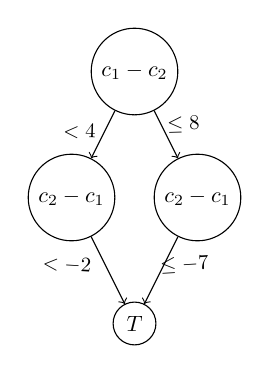
\begin{tikzpicture}[
		smallvertex/.style={circle,draw,scale=0.8}
		]
			
		\node[smallvertex](S0){$c_1 - c_2$};
		\node[smallvertex, below of = S0, yshift = -1 cm, xshift = -1 cm](S1){$c_2 - c_1$};
		\node[smallvertex, below of = S0, yshift = -1 cm, xshift = 1  cm](S2){$c_2 - c_1$};
		\draw[->] (S0) --(S1) node [midway, above, sloped, scale=0.75,
		rotate=295, xshift =-0.4 cm, yshift = -0.2cm]{$<4$};
		\draw[->] (S0) --(S2) node [midway, above, sloped, scale=0.75,
		rotate=65, xshift =0.3 cm, yshift = -0.1cm]{$\leq 8$};
		\node[smallvertex, below of = S0, yshift = -3cm](S3){$T$};
		\draw[->] (S1) --(S3) node [midway, above, sloped, scale=0.75,
		rotate=60, xshift =-0.7 cm, yshift = -0.2cm]{$<-2$};
		\draw[->] (S2) --(S3) node [midway, above, sloped, scale=0.75,
		rotate=300, xshift =0.4 cm, yshift = -0.2cm]{$\leq-7$};
	\end{tikzpicture}
	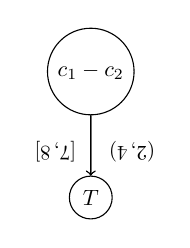
\begin{tikzpicture}[
		smallvertex/.style={circle,draw,scale=0.8}
		]
			
		\node[smallvertex](S0){$c_1 - c_2$};
		\node[smallvertex, below of = S0, yshift = -1cm](S3){$T$};
		\draw[->] (S0) --(S3) node [midway, above, sloped, scale=0.75,
		rotate=90, xshift =-0.7 cm, yshift = -0.2cm]{$(2,4)$};
		\draw[->] (S0) --(S3) node [midway, above, sloped, scale=0.75,
		rotate=90, xshift =0.6 cm, yshift = -0.2cm]{$[7,8]$};
	\end{tikzpicture}	
	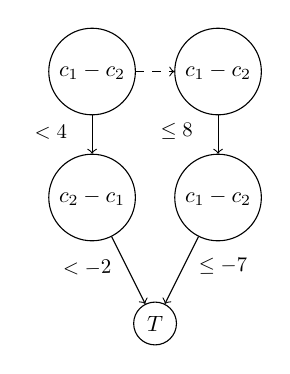
\begin{tikzpicture}[
		smallvertex/.style={circle,draw,scale=0.8}
		]
			
		\node[smallvertex](S0){$c_1 - c_2$};
		\node[smallvertex, right of = S0, xshift = 1cm](S1){$c_1 - c_2$};
		\draw[dashed,->] (S0) --(S1) node [midway, above, sloped, scale=0.75,
		rotate=0, xshift =-0.7 cm, yshift = -0.2cm]{};
		\node[smallvertex, below of = S0, yshift = -1cm](S2){$c_2 - c_1$};
		\draw[->] (S0) --(S2) node [midway, above, sloped, scale=0.75,
		rotate=90, xshift =-0.7 cm, yshift = -0.2cm]{$< 4$};
		\node[smallvertex, below of = S1, yshift = -1cm](S3){$c_1 - c_2$};
		\draw[->] (S1) --(S3) node [midway, above, sloped, scale=0.75,
		rotate=90, xshift =-0.7 cm, yshift = -0.2cm]{$\leq 8$};
		\node[smallvertex, below of = S0, xshift = 1cm, yshift = -3cm](S4){$T$};
		\draw[->] (S2) --(S4) node [midway, above, sloped, scale=0.75,
		rotate=65, xshift =-0.7 cm, yshift = -0.2cm]{$<-2$};
		\draw[->] (S3) --(S4) node [midway, above, sloped, scale=0.75,
		rotate=297, xshift =0.7 cm, yshift = -0.2cm]{$\leq-7$};
	\end{tikzpicture}
	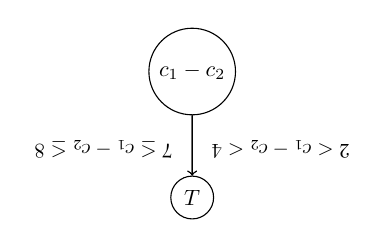
\begin{tikzpicture}[
		smallvertex/.style={circle,draw,scale=0.8}
		]
			
		\node[smallvertex](S0){$c_1 - c_2$};
		\node[smallvertex, below of = S0, yshift = -1cm](S3){$T$};
		\draw[->] (S0) --(S3) node [midway, above, sloped, scale=0.75,
		rotate=90, xshift =-1.5 cm, yshift = -0.2cm]{$2<c_1-c_2<4$};
		\draw[->] (S0) --(S3) node [midway, above, sloped, scale=0.75,
		rotate=90, xshift =1.5 cm, yshift = -0.2cm]{$7\leq c_1-c_2\leq8$};
	\end{tikzpicture}	
	
\end{center}
\caption{A CRD, CDD, DDD and CMD representation}
\label{fig:Diagrams}
\end{figure}

\begin{table}[]
\centering
\label{table:diagrams}
\begin{tabular}{|l|l|l|}
\hline
DMB                                                    & \begin{tabular}[c]{@{}l@{}}Canonical form for convex zones\\ Existing library\\ Inclusion check\end{tabular}                                                                                                                                                                                & \begin{tabular}[c]{@{}l@{}}Concave zones need multiple DBMs\\ Not memory efficient\end{tabular}                                                                                                                                              \\ \hline
DDD                                                    & \begin{tabular}[c]{@{}l@{}}Nodes with difference constraints\\ Implement as LDD \\ Re-ordering of variables possible\\ Apply same efficiency as BDDs\\ Boolean variables also in DDD\end{tabular}                                                                                           & \begin{tabular}[c]{@{}l@{}}Canonicity hard to obtain\\ No on the fly canonicity\\ Only speed performance tested\\ Only reduction algorithms\end{tabular}                                                                                     \\ \hline
CDD                                                    & \begin{tabular}[c]{@{}l@{}}Branching on intervals\\ Implement as MDD\\ Intervals need to be disjoint\\ Inclusion check\\ (intersection of complement)\end{tabular}                                                                                                                          & \begin{tabular}[c]{@{}l@{}}No algorithm to get normal form\\ Only high level algorithms\\ Methods don't maintain disjointness\\ Expensive normal form computation\\ No implementation results\\ Disjointness memory inefficient\end{tabular} \\ \hline
CRD                                                    & \begin{tabular}[c]{@{}l@{}}Nodes with multiple fanout for \\ upperbound constraints\\ Combination with BDD possible\\ Variable ordering with \\ interleaving is best\\ Modelchecker available\\ Library available\\ Some benchmarks exp better than CDD\\ Extensive benchmarks\end{tabular} & \begin{tabular}[c]{@{}l@{}}3 possible canonical forms\\ Good performance backwards reach\\ No algorithms in paper\\ Some benchmarks linear worse than CDD\end{tabular}                                                                       \\ \hline
CMD                                                    & \begin{tabular}[c]{@{}l@{}}Multiple DBM constraints per edge\\ Benchmarks against RED and UPPAAL\end{tabular}                                                                                                                                                                               & \begin{tabular}[c]{@{}l@{}}Results differ per case\\ Needs translation from vector to edges\\ Two reduced forms\end{tabular}                                                                                                                 \\ \hline
\begin{tabular}[c]{@{}l@{}}BDD\\ discrete\end{tabular} & \begin{tabular}[c]{@{}l@{}}Using existing BDD packages\\ Good performance for small clock values\end{tabular}                                                                                                                                                                               & \begin{tabular}[c]{@{}l@{}}Performance decreases fast for large values\\ Not possible with current opaal PINS\\ Models created separately as C code\\ Introducing 'tick' actions\\ Only for closed timed automata\end{tabular}               \\ \hline
\begin{tabular}[c]{@{}l@{}}BDD\\ zones\end{tabular}    & \begin{tabular}[c]{@{}l@{}}Using existing BDD packages\\ All variable reorderings possible\\ Only need direct translation DBM to\\ state vector\\ Easy to implement\end{tabular}                                                                                                            & \begin{tabular}[c]{@{}l@{}}Losing zone containment\\ No implementation results\end{tabular}                                                                                                                                                  \\ \hline
\end{tabular}
\end{table}

A known difficulty in BDDs is the variable ordering. A bad ordering can lead to a BDD exponential in size where a good ordering can sometimes lead to a significant smaller diagram. Of the diagrams named above only CRDs have experimented with different orderings, the other researches assume a given ordering on the variables and the ordering of the values is fixed. The CRD case shows that full interleaving and having related variables close to each other in the ordering is preferable and gives the best results, both on speed and memory. This is the same result as expected with BDDs, this suggests that similar orderings should be used with these techniques.

\begin{figure}[t] 
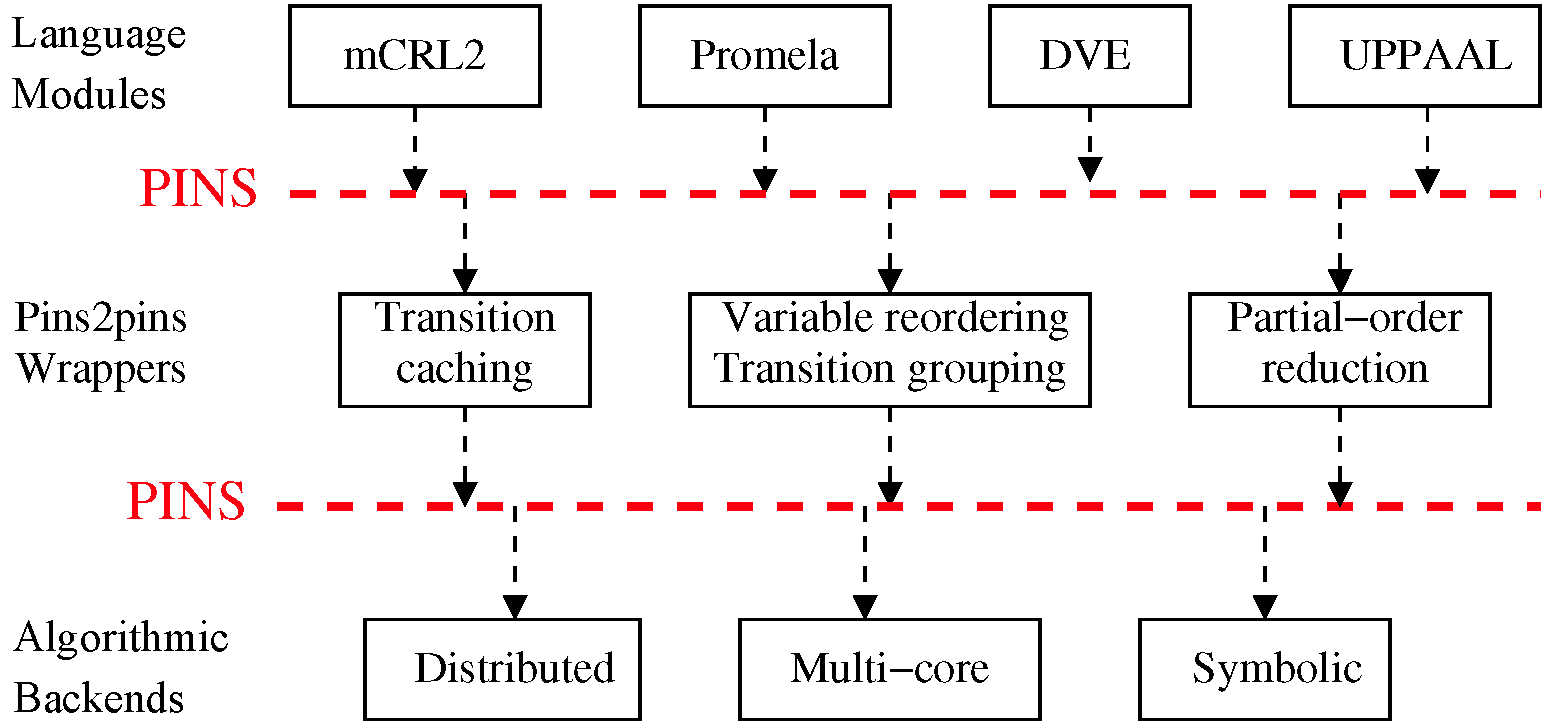
\includegraphics[width=\textwidth]{pins_modern}
\caption{Modular structure of LTSmin}
\label{fig:pins_modern}
\end{figure}

LTSmin~\cite{eemcs18152,ltsmin-mc:nmf2011} is a language independent model checker. It is build in a modular way such that new languages can be added by an PINS interface without too much effort, and new algorithms can be added more easily. LTSmin offers four different algorithmic back ends for model analysis: symbolic, multi-core, sequential and distributed. All of these back ends support different types of reduction and model checking. Several language modules have already been built for LTSmin such as mCRL2, Promela, DVE and UPPAAL. The modular structure of LTSmin is shown in figure \ref{fig:pins_modern}. States are stored in fixed length integer arrays. The PINS(Partitioned Next-State Interface) is the core of LTSmin. This interface abstracts as much as possible from the model without losing the structure. The main function of the interface is a (partitioned) next state function which returns the successor states. With these functions a state space can be generated on the fly. With the use of dependency matrices event locality can be determined statically~\cite{rwcmatrices}. Using these matrices, more efficient symbolic algorithms can be used, the number of next-state calls can be reduced and transition caching can be used. In the current UPPAAL PINS the next-state function is not partitioned and therefore no meaningful dependency matrix is created, and all of these algorithms can not be used.

\subsection{Timed Automata}
Timed Automata is a formalism that extends labelled transition systems with one ore more, but finite, clocks. As our work continues on ~\cite{eemcs21972} we use the same definition of timed automata.
\begin{mydef}[Timed Automata]
\label{def:TA}
An extended timed automaton is a 7-tuple A = $<L, C, Act, s_0, \rightarrow, I_c>$ where
{\renewcommand\labelitemi{--}
	\begin{itemize}
		\item L is a finite set of locations, typically denoted by $l$
		\item C is ia finite set of clocks, typically denoted by c
		\item Act is a finite set of actions
		\item $s_0 \in$ L is the initial location
		\item $\rightarrow \subseteq L \times G(C) \times Act \times 2^C \times L$ is the (non-deterministic) transition relation. We noramlly write l $\stackrel{g,a,r}{\longrightarrow}$ l' for a transition., where l is the source location, g is the guard over the clocks, a is the action, and r is the set of clocks reset.
		\item $I_C : L \rightarrow G(C)$ is a function mapping locations to downwards closed clock invariants.
	\end{itemize}
}
\end{mydef}

With this definition we can combine timed automata to a network of timed automata to define larger systems.

\begin{mydef}[Network of timed automata~\cite{eemcs21972}]
\label{def:networkTA}
Let Act = $\{ch!,ch?|ch \in Chan\} \cup \{\tau\}$ be a finite set of actions, and let C be a finite set of clocks. Then the parallel composition of extended timed automata $A_i = (L_i, C, Act, S^i_0, \rightarrow_{i}, I^i_C)$ for all $1 \leq i \leq n$, where $n \in \mathbb{N}$, is a network of timed automata, denoted $A = A_1||A_2||..||A_n$.
\end{mydef}

\subsection{Zones}
For basic transition systems the state space can grow exponentially for the size of the system. For Timed Automata the growth can become even larger and in some cases become unbounded by the addition of clocks. To tackle this problem most model checkers use a notion of zones for the representation of time. A zone can be seen as a set of constraints over the clocks C of the form $c_i \sim x$ and $c_i - c_j \sim x$ where $\sim  \in \{<, \leq, =, \geq, >\}$ and $x \in \mathbb{N}$. To represent these zones several data structures have been developed. One of the most common used structures are Difference Bound Matrices(DBMs)~\cite{dbmorig,bengtsson2002clocks}.
 
These matrices use both a column and a row for each clock, and on each position $(i,j)$ an upper bound on the difference between the clocks $c_i$ and $c_j$ is given in the form $c_i - c_j \preceq x$ where $\preceq \in \{<, \leq\}$ and $x \in \mathbb{N}$. For the constraints over the single clocks an extra clock $\mathbf{O}$ with a constant value 0 is added. By switching the two variables also a lower bound can be given to each pair. This way convex zones of clock variables can be represented. Each matrix can however only contain a single convex zone. Concave zones and multiple convex zones need multiple matrices to be represented. As a solution often a list of DBMs is used. 

\section{Plan}

\subsection{Questions}
For the research we will state a couple of research questions:
{\renewcommand\labelitemi{--}
	\begin{itemize}
		\item Is the combination of BDDs and DMBs an efficient method for model checking timed automata?
		\item Can improvements be achieved by different orderings? Both by changing the order of only the clock variables and by mixing the clock and state variables.
		\item Is the new PINS needed for the symbolic approach also usable for the multicore approach?
		\item Can the BDD approach be generalized towards DDDs?
	\end{itemize}
}

\subsection{Approach}
To answer the questions stated above we will first create a model checker for timed automata based on BDDs. We will use a zone representation of the clock variables. We will calculate the zone representation using DBMs in the next state generation. To do this we will adapt the current opaal PINS. We will also test this new PINS with the current multicore tool. T

%\subsection{Approach}
%The first task will be to find a suitable translation function from DBM values to integers that LTSmin uses as state vector, and vice versa. This function will be needed at the begin and end of each next-state call. Together with this the structure of the UPPAAL PINS will need to be changed. For the later experiments also changes to the ordering of variables and a partition of the next state function in the PINS will be constructed. 

%For the tests on variable ordering heuristics we will use the options that have already been implemented in LTSmin~\cite{rwcmatrices}. We will compare these against the basic ordering and the manually created orderings. For this experiment also the partitioned next state function will be needed as otherwise no meaningful dependency matrices exist and no reordering can be performed. 

%We will test all our approaches with multiple testcases against the state of the art UPPAAL and the latest multi core version of LTSmin. All tests will be carried out on a laptop with 4GB of memory and a 2.53GHz Intel I5 processor with 4 cores. If we achieve promising results, the tests can be expanded to a 48 core machine, on which the multi threaded algorithms can be exploited more and thus better tests on time efficiency can be performed.
%The fist task will be to change the opaal PINS to no longer use pointers to DBMs, but to add the DBM directly into the state vector. 

\subsection{To do}
In this section we describe all things that need to be implemented to make model checking with a certain diagram possible. 

To make symbolic model checking work we need to change the opaal PINS. The PINS currently uses a pointer to a DBM. For the new approach we will put the values of the DBM directly into the state vector. This will increase the size of the state vector. All other references to the types and values of the state vector entries will need to be changed also. 

To make symbolic variable reordering possible we will need to partition the next state function and create a dependency matrix. In the code the next state function is already split up per transition, but in a single transition group. Splitting this into multiple transition groups should not be too hard. In this same step also the dependency matrices need to be created and made as sparse as possible.

To combine the new PINS with the multicore LTSmin backend the subsumption check will need to be changed. This check now relies on a pointer to a DBM, but it will now get the complete DBM, or state vector. Here the search algorithm or the subsumption check will need to know which variables are zone variables. It will also occur that different states will have the same discrete variables, but different zone variables, these all need to be checked for the subsumption check.

For the combination with the multicore backend also the data structure will need to be adapted. The current structure stores a discrete state together with a set of pointers to DBMs. In the new situation each pair of discrete state and DBM will be stored explicitly.

For the DDD the diagram will need to be able to identify the zone variables from the discrete state variables in the state vector. This will need an extra function in the PINS interface. This function will also need to cope with variable reordering. 

For the DDD representation the values from the DBM will need to be translated to useful variables as ordering based on values is needed. Also to check for inequalities and set containment the meaningful values are needed. As the values in a DBM both contain the value of an inequality and the operator some more complex translation might be needed. 

%For the CMD a technique will be needed to map the values from the state vector to the edges of the diagram. For all other diagrams the values can be put into nodes in the same order as the vector. For the CMD the ordering can change throughout the diagram. 

For the DDD the mixing of BDDs and zone diagrams need to be researched. There is little knowledge on how algorithms might need to be changed. Also the possibility of the mixing of discrete and zone variables need to be researched. It might be that it functions better when the two types of variables remain separated, or when they are mixed.

\subsection{Planning}

\bibliography{references}{}
\bibliographystyle{unsrt}
\end{document}